\begin{figure}[H]
  \begin{adjustwidth}{-12mm}{-12mm}
  \begin{subfigure}[b]{0.3\textwidth}
  \centering
  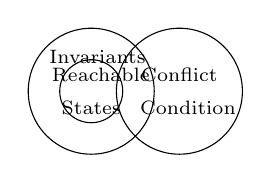
\begin{tikzpicture}[scale=0.4]

    \draw (0,0) circle (1cm) node[text width=1cm,align=center]{\ti{\scriptsize Reachable \\  States}};
  \draw (0,0) circle (2cm) ++(0.2,1.6)node[below]{\ti{\scriptsize Invariants}};
  \draw (2.8,0) circle (2cm) node[text width=1cm,align=center]{\ti{\scriptsize Conflict \\ Condition}};
  \end{tikzpicture}
  \caption{Real conflict}\label{fig:r1}
  \end{subfigure}
  \hspace{7mm}
  \begin{subfigure}[b]{0.3\textwidth}
  \centering
  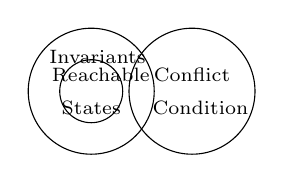
\begin{tikzpicture}[scale=0.4]

  \draw (0,0) circle (1cm) node[text width=1cm,align=center]{\ti{\scriptsize Reachable \\ States}};
  \draw (0,0) circle (2cm) ++(0.2,1.6)node[below]{\ti{\scriptsize Invariants}};
\draw (3.2,0) circle (2cm) node[text width=1cm,align=center]{\ti{\scriptsize Conflict \\ Condition}};
  \end{tikzpicture}
  \caption{False-conflict not }\label{fig:r2}
  \end{subfigure}
  \hspace{10mm}
  \begin{subfigure}[b]{0.3\textwidth}
  \centering
  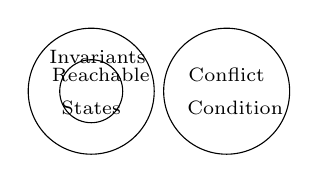
\begin{tikzpicture}[scale=0.4]

  \draw (0,0) circle (1cm) node[text width=1cm,align=center]{\ti{\scriptsize Reachable \\ States}};
  \draw (0,0) circle (2cm) ++(0.2,1.6)node[below]{\ti{\scriptsize Invariants}};
  \draw (4.3,0) circle (2cm) node[text width=1cm,align=center]{\ti{\scriptsize Conflict \\  Condition}};
  \end{tikzpicture}
  \caption{False-conflict}\label{fig:r3}
  \end{subfigure}
\end{adjustwidth}
  \caption{Different cases of conflict detection}\label{fig:reach}

\end{figure}
